\subsection{Architecture}

The MVC schema for the client can be seen in figure
\ref{fig:client_architecture}.

\begin{figure}[h]
	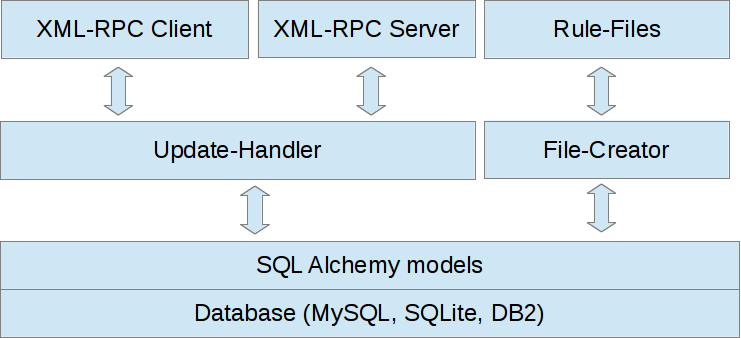
\includegraphics[width=130mm]{./img/Client-MVC.png}
	\caption{Client Architecture}
	\label{fig:client_architecture}
\end{figure}

The update handler of the client have both a XML-RPC Client and a XML-RPC
Server. The XML-RPC Client is used to connect to the central server to do a
rule synchronization. The XML-RPC Server is here so that the central server can
connect to the client and check to see if the client is alive or to order
the client to do a rule syncronization.

As the client should be as light weight as possible and the only thing we from
any framework on it is a simple database connection and abstraction layer, we
have decided to not use \django{} for the client. Instead we use the database ORM
\cite{database_orm} for Python called SQL-Alchemy \cite{sql_alchemy}, which is a
much more light weight than \django{} for this purpose.

The client also contains a file creator which takes the rules objects in the
database and generates the files Snort needs in the format Snort needs them in.
